%
%
 The unsteady, compressible, Favre-averaged Navier-Stokes
 equations for a blade row in 3D can be cast in terms of
 absolute velocity $\vec{v}$ but solved in a relative non-Newtonian reference frame
 rotating along with the blade about the $x$ axis with angular velocity
 ${\bf \Omega}$ as shown in Fig. \ref{axis.fig}.
 This system of equations, written in a dimensionless, Arbitrary
 Lagrangian-Eulerian (ALE), integral conservative
 form (Donea et al. \citeyearNP{Donea}) for a control
 volume ${\cal V}\left(t\right)$ with boundary
 ${\cal S}\left(t\right)$
 in Cartesian coordinates $\vec{x} = \left(x, y, z\right)$,
 takes the form
%
\beq
  \fpdt{} \int_{{\cal V}\left(t\right)} {\bf U} d{\cal V} +
  \oint_{{\cal S}\left(t\right)} \left[
  \vec{{\bf F}} \left({\bf U}, \vec{u}\right) -
  \frac{1}{Re}\vec{{\bf G}} \left({\bf U}, \nabla {\bf U}\right) \right]
  \cdot\vec{n}\, d{\cal S} =
  \int_{{\cal V}\left(t\right)} {\bf S}\,d{\cal V}
  \label{conservative_formulation_nl.eq}
\eeq
%
%
\begin{figure}[ht]
  \centerline{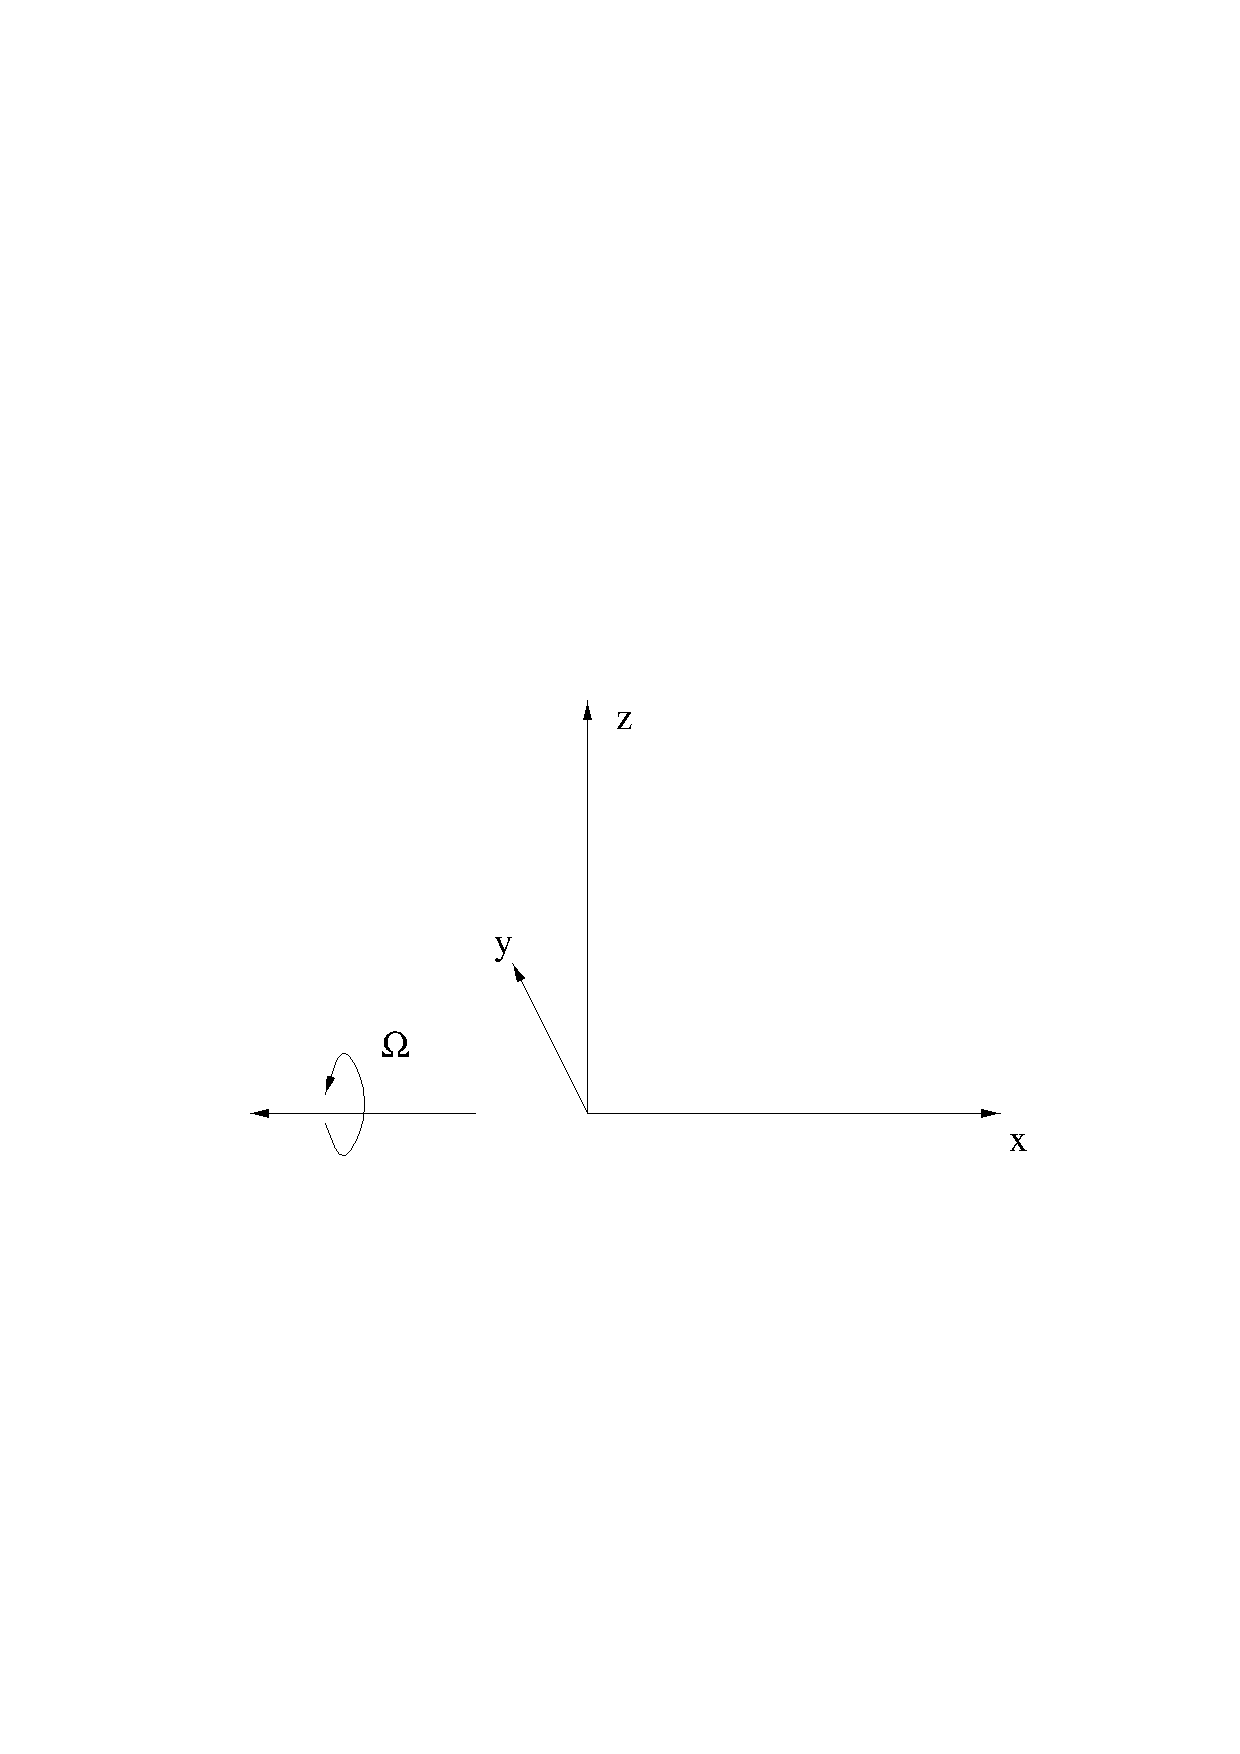
\includegraphics[width=60mm,clip=t]{CHAP_NONLIN/FIGURE/axis.pdf}}
  \caption{Direction of blade rotation}
  \label{axis.fig}
\end{figure}
%
 The viscous term $\vec{\bf G}$
 on the left-hand side of (\ref{conservative_formulation_nl.eq})
 is scaled by the reference Reynolds number so that flow variables are
 non-dimensionalised consistently. The dimensionless quantities are evaluated
 from their dimensional counterparts using the dimensional reference values
 reported in Appendix \ref{nondim.chap}.
 $\vec{n}$ represents the outward unit vector of the control volume boundary
 ${\cal S}\left(t\right)$. The vector $\vec{u}$, which represents the
 velocity in the relative frame of reference minus the velocity
 $\frac{d \vec{x}}{d t}$ of the boundary
 ${\cal S}\left(t\right)$, can be written as:
%
\beq
   \vec{u} = \vec{v} - \vec{\Omega} \times \vec{x} - \frac{d \vec{x}}{d t}
   \label{relative_velocity.eq}
\eeq
%
 where $\vec{\Omega} = \left(-\Omega,0,0\right)$. The sign of the angular velocity vector
 is determined by the assumption that the positive rotational speed is the
 one indicated in Fig. \ref{axis.fig}.
 The solution vector of conservative variables ${\bf U}$ is given by:
%
\beq
   {\bf U} = \left[
   \begin{array}{ccccc}
   \rho & \rho v\sm{1} & \rho v\sm{2} & \rho v\sm{3} & \rho E
   \end{array}
   \right]\se{T}
   \label{conservative_variables.eq}
\eeq
%
 The inviscid flux vector  $\vec{{\bf F}}\left({\bf U}, \vec{u}\right)$
 has the following components\footnote{${\bf U}u\sm{j}$ represents the $j$ component
 of the convective flux, while ${\bf F}{\scriptstyle p}\sm{j}$ represents the $j$ component
 of the pressure flux.}:
%
\beq
   {\bf F}\sm{j} &=& {\bf U}u\sm{j} + {\bf F}{\scriptstyle p}\sm{j}
   \label{nonlinear_inviscid_flux.eq}\\
   {\bf F}{\scriptstyle p}\sm{j} &=&
   \left[
   \begin{array}{ccccc}
   0 & p\delta\sm{1j} & p\delta\sm{2j} & p\delta\sm{3j} & v\sm{j} p
   \end{array}
   \right]\se{T}
   \label{nonlinear_pressure_flux.eq}
\eeq
%
 where $\delta\sm{ij}$ represents the Kronecker delta function.
 The static pressure $p$ and the total energy $E$ are related, in
 a non-dimensional fashion, to the density
 $\rho$, absolute velocity $\vec{v}$ and total enthalpy $H$
 by the following two equations which assume perfect gas with a constant
 ratio $\gamma$ of specific heat.

%
\beq
  p = \left(\gamma - 1\right) \rho \left[E - \frac{\left|\vec{v}\right|\se{2}}{2}\right],
  \ \ \ \ \ \
  H = E + \frac{p}{\rho}
 \label{pressure_energy_relations.eq}
\eeq
%
 Following the approach of Sbardella \& Imregun \citeyear{Luca:7,Luca:11},
 the viscous part of the governing equations is split into
 two distinct components, namely:

%
\beq
 \vec{\bf G} = \vec{\bf G}{\scriptstyle l} + \vec{\bf G}{\scriptstyle m}
 \label{viscous_terms.eq}
\eeq
%
 where

%
\beq
 \vec{\bf G}{\scriptstyle l} = \left[
 \begin{array}{c}
  0 \\ \mu \nabl v\sm{1} \\
       \mu \nabl v\sm{2} \\
       \mu \nabl v\sm{3} \\
       \mu\sum\sm{j=1}\se{3} v\sm{j}\nabl v\sm{j}
      + \frac{\gamma}{\gamma\!-\!1}
       \left(\frac{\mu\sm{l}}{Pr\sm{l}}\!+\!\frac{\mu\sm{t}}{Pr\sm{t}}\right) \nabl T
 \end{array} \right]
 \label{mean_flow_laplacian.eq}
\eeq
%
 $T=p/\rho$ is the non-dimensional static temperature of the fluid.
 The $j$-component of the second term on the left-hand side of
 (\ref{viscous_terms.eq}) is:

%
\beq
 {\bf G}{\scriptstyle m}\sm{j} = \left[
 \begin{array}{c}
  0 \\ \mu \fpd{v\sm{j}}{x\sm{1}} +
       \left(\lambda\nabl\cdot\vec{v}\right)\delta\sm{1j}\\
       \mu \fpd{v\sm{j}}{x\sm{2}} +
       \left(\lambda\nabl\cdot\vec{v}\right)\delta\sm{2j}\\
       \mu \fpd{v\sm{j}}{x\sm{3}} +
       \left(\lambda\nabl\cdot\vec{v}\right)\delta\sm{3j}\\
       \mu\left(\vec{v}\cdot\nabl v\sm{j}\right) +
       \lambda v\sm{j}\left(\nabl\cdot\vec{v}\right)
 \end{array} \right]
 \label{mean_flow_mixed.eq}
\eeq
%
 In (\ref{mean_flow_laplacian.eq}) and (\ref{mean_flow_mixed.eq}),
 $\mu$ represents the total dynamic viscosity of the fluid and is given
 by the summation of the laminar (physical) dynamic viscosity $\mu\sm{l}$
 and the turbulent dynamic viscosity $\mu\sm{t}$.
 The value of $\lambda$ is given by the
 Stokes relation $\lambda = -\frac{2}{3} \mu$
 which is valid for the majority of the flow situations with the exception
 of very high temperature or pressure ranges.
 It is easily seen that the
 component $\vec{\bf G}\sm{l}$ in (\ref{mean_flow_laplacian.eq})
 includes  the Laplacian operators of the three velocity components and
 temperature only.
 The second component, $\vec{\bf G}\sm{m}$, contains the mixed derivative terms,
 while the vector of source terms ${\bf S}$ on the right-hand side of
 (\ref{conservative_formulation_nl.eq}) takes into accounts for the blade
 rotation

%
\beq
  {\bf S} = \left[
   \begin{array}{ccccc}
    0 & 0 & \rho \Omega v\sm{3} & -\rho \Omega v\sm{2} & 0
   \end{array}
   \right]\se{T}
   \label{source_term.eq}
\eeq
%
 The derivation of the constitutive relations of viscous flows is discussed
 in detail by Schlichting \citeyear{Schlichting} and White \citeyear{White:1}.
